\chapter{KBBQ: A reference-free method for base quality score recalibration}
\label{ch:kbbq}
\section{Introduction}

Next generation sequencing has a plethora of applications in biology. %TODO: give some examples
While the technology is widely applied, the sequencing process is inherently erroneous and errors are common in sequencing data, with base substitution error rate estimates ranging between $.1$ and $1\%$, depending on the sequencing technology used \parencite{fox_accuracy_2014}.
To help mitigate this, DNA molecules are usually copied and sequenced multiple times to ensure the sequence is correct, since multiple independent measurements are unlikely to all contain the same error at the same position. While this works well in general, it can be costly and additional sample manipulation can damage samples and insert mutations, further increasing the amount of technical error in the data \parencite{schirmer_insight_2015, ma_analysis_2019}.

\subsection{Quality Scores}

In addition to increased sequencing depth, quality scores are an important part of sequencing data that helps identify erroneous sequences. Sequencing data is usually presented along with quality scores in the Phred scale \parencite{ewing_base-calling_1998, ewing_base-calling_1998-1}.
These quality scores measure the confidence the instrument has in its determination that any particular base in the sequence is correct.
Specifically, the quality score is equal to $-10\log_{10}P(e)$ \parencite{ewing_base-calling_1998,ewing_base-calling_1998-1}, where $P(e)$ is the probability the base is an error.
For example, a base with a quality score of 40 has a .0001 probability of being incorrect while a base with a quality score of 10 has probability .1 of being incorrect. Generally, bases with scores lower than 10 are considered bad quality and bases with scores 30 and above are considered to be good quality. However, the score allows finer resolution than ``good'' and ``bad'', and is therefore more nuanced.

%new paragraph - importance
The usefulness of quantitative scores over categorical can be illustrated by considering how variant calling algorithms utilize quality scores.
Variant calling is a task to identify genetic variation in a sample from sequencing data.
Variant calling models use quality scores to differentially weight the observed data. Generally, these models attempt to find the sample genotype most consistent with the observed data and recognize that low quality bases provide less reliable evidence for one genotype over another. The BCFTools multiallelic caller \parencite{li_sequence_2009}, GATK's HaplotypeCaller \parencite{poplin_scaling_2018}, and FreeBayes \parencite{garrison_haplotype-based_2012}---three of the most popular variant callers---all take quality score into consideration when calling variants.
Since the quality score is an exactly defined probability, it is straightforward to integrate these scores into a model.

%new paragraph - binning
If so desired, quantitative scores can be collapsed into coarser categories, such as ``good'' and ``bad''. This is sometimes done as a heuristic; \textit{ie.}\ scores less than 10 are untrustworthy and filtered out of a dataset and other scores are trusted and retained.
The practice of binning quality scores together with neighboring scores is commonly performed to reduce file size \parencite{shibuya_better_2019, malysa_qvz_2015, yu_quality_2015, noauthor_reducing_2014}. 
However, it's important to note that this process cannot be simply reversed as information is lost when the scores are binned.

\subsection{Base Quality Score Recalibration}

% What is Base Quality Score Recalibration?
While base quality scores are important for identifying reliable data, base quality scores are often incorrect.
Base quality scores are exactly defined as a probability. They can be interpreted as a prediction giving the probability the reported base is an error. In general, probabilities are called \textit{calibrated} if the reported probability accurately predicts the frequency of an event.
Base quality scores in Illumina sequencing reads are not well-calibrated \parencite{callahan_dada2:_2016, ni_improvement_2016}. %(TODO: more cites)
A few alternative base calling models have been developed for Illumina machines that improve base call accuracy and quality score calibration; however, these are difficult to use because they require the raw output from the sequencing machine, which is unavailable to most users of sequencing as they are usually disposed of after a sequencing run due to the large cost associated with storing that data \parencite{kao_naivebayescall_2011, massingham_all_2012}. 


Since base quality scores are used to some degree by most variant calling methods, it is probable that poorly calibrated reads reduce the quality of resulting variant calls.
Similarly, the reduced amount of information in binned quality scores may also impact the quality of variant calls made using the data.
Poor calibration combined with poor resolution resulting from quality score binning may have an important impact on algorithms that rely on these scores to function, but the exact effect of these phenomena are unknown.

%actual BQSR
Though increased sequencing depth can help mitigate the impact of random sequencing errors, sequencing is affected by non-random biases.
For these types of errors, increasing sequencing depth counterintuitively \textit{increases} the effect of these errors, as they by definition occur preferentially at the same location. Thus, increased sequencing depth at that location adds more errors than are expected by chance, making those erroneous reads seem trustworthy. 
These biases can be due to the nature of the DNA sequence itself, with errors induced during library preparation or the sequencing reaction likely due to secondary structure \parencite{meacham_identification_2011, nakamura_sequence-specific_2011, schirmer_insight_2015, ma_analysis_2019}.
At the same time, the sequencing reaction is also non-randomly biased. Bases at the end of a read are much more likely to be erroneous than bases at the beginning of the read, and the identity of the base and adjacent bases also affect the error rate \parencite{fox_accuracy_2014, schirmer_illumina_2016}. 
Thus while random errors are troublesome, their impacts can be somewhat mitigated by more sequencing. Systematic errors cannot addressed in the same way, but they can be modeled and incorporated into quality scores.
%discuss non-random genomic locus vs. sequencing characteristics etc.    %non-random errors

% GATK BQSR occurs in 3 phases.
% Phase 1 - Count errors and covariates
Base quality score recalibration (BQSR) is the process of modeling errors in sequencing data and using the created model to update quality scores such that they reflect an accurate probability of error of any base.
GATK BQSR  is the most popular method for BQSR and is recommended before variant calling by the GATK best practices \parencite{auwera_fastq_2013}.
The model integrates many covariates of error such that the output quality score reflects an accurate, independent measure of the probability of error.
The algorithm takes reads aligned to a reference and a database of potentially variable sites in the genome as input.

The algorithm proceeds in 3 phases.
In the first phase, the algorithm compares each read to the aligned reference. Potentially variable sites are ignored and mismatches from the reference sequence and non-mismatches are counted. The numbers of matching and mismatching bases are categorized according to the model covariates, which are: read group, assigned quality score, sequencing cycle, and the base identity along with the identity of the previous base (the base context).
% Phase 2 - Train a hierarchical model.
In the second phase, a bayesian hierarchical model is trained with the count data. Using a normal distribution of the mean probability of error as a prior, the \textit{maximum a posteriori} (MAP) quality score of the read group is calculated assuming the errors are binomially distributed. The estimated error probability for each read group $\hat{Q}_{rg}$ can be written in terms of the binomial probability mass function $\mathcal{B}$ with error probability $Q_{rg}$ and number of observations $\operatorname{Observations}_{rg}$ and the normal probability density function $\mathcal{N}$ with standard deviation of 1 around the mean estimate of the quality score for the entire dataset, $\bar{Q}$
\begin{align}
\hat{Q}_{rg} &= \operatorname{argmax}_{Q_{rg}} P(Q_{rg}|\operatorname{Errors}_{rg}) \\
&= \operatorname{argmax}_{Q_{rg}} P(\mathcal{B}(\operatorname{Errors}_{rg} | \operatorname{Observations}_{rg}, Q_{rg}) \times P(\mathcal{N}(Q_{rg} | \bar{Q}))
\end{align}
This score is then used as the prior for calculating the \textit{maximum a posteriori} quality score for each assigned quality score in that read group, $\hat{Q}_{\operatorname{assigned\:quality\:score}}$, using a similar formula.
In turn, this score is used as the prior for calculating the \textit{maximum a posteriori} scores for the sequencing cycle and context covariates of bases with that score. The difference between the MAP estimate and the prior is used to calculate the final score, which is the sum of the MAP estimate of the assigned quality score and these two differences. That is,
\begin{align}
\Delta Q_{\operatorname{cycle}} &= \hat{Q}_{\operatorname{cycle}} - \hat{Q}_{\operatorname{assigned\:quality\:score}} \\
\Delta Q_{\operatorname{context}} &= \hat{Q}_{\operatorname{context}} - \hat{Q}_{\operatorname{assigned\:quality\:score}} \\
Q_{\operatorname{recalibrated}} &= \hat{Q}_{\operatorname{assigned\:quality\:score}} + \Delta Q_{\operatorname{cycle}} + \Delta Q_{\operatorname{context}}
\end{align}
In the third phase, the quality score of each read is adjusted based on the four covariates for each base in the read according to values calculated in the previous phase. See Figure \ref{fig:recal_explain} for a visual example.

\begin{figure}
\centering
	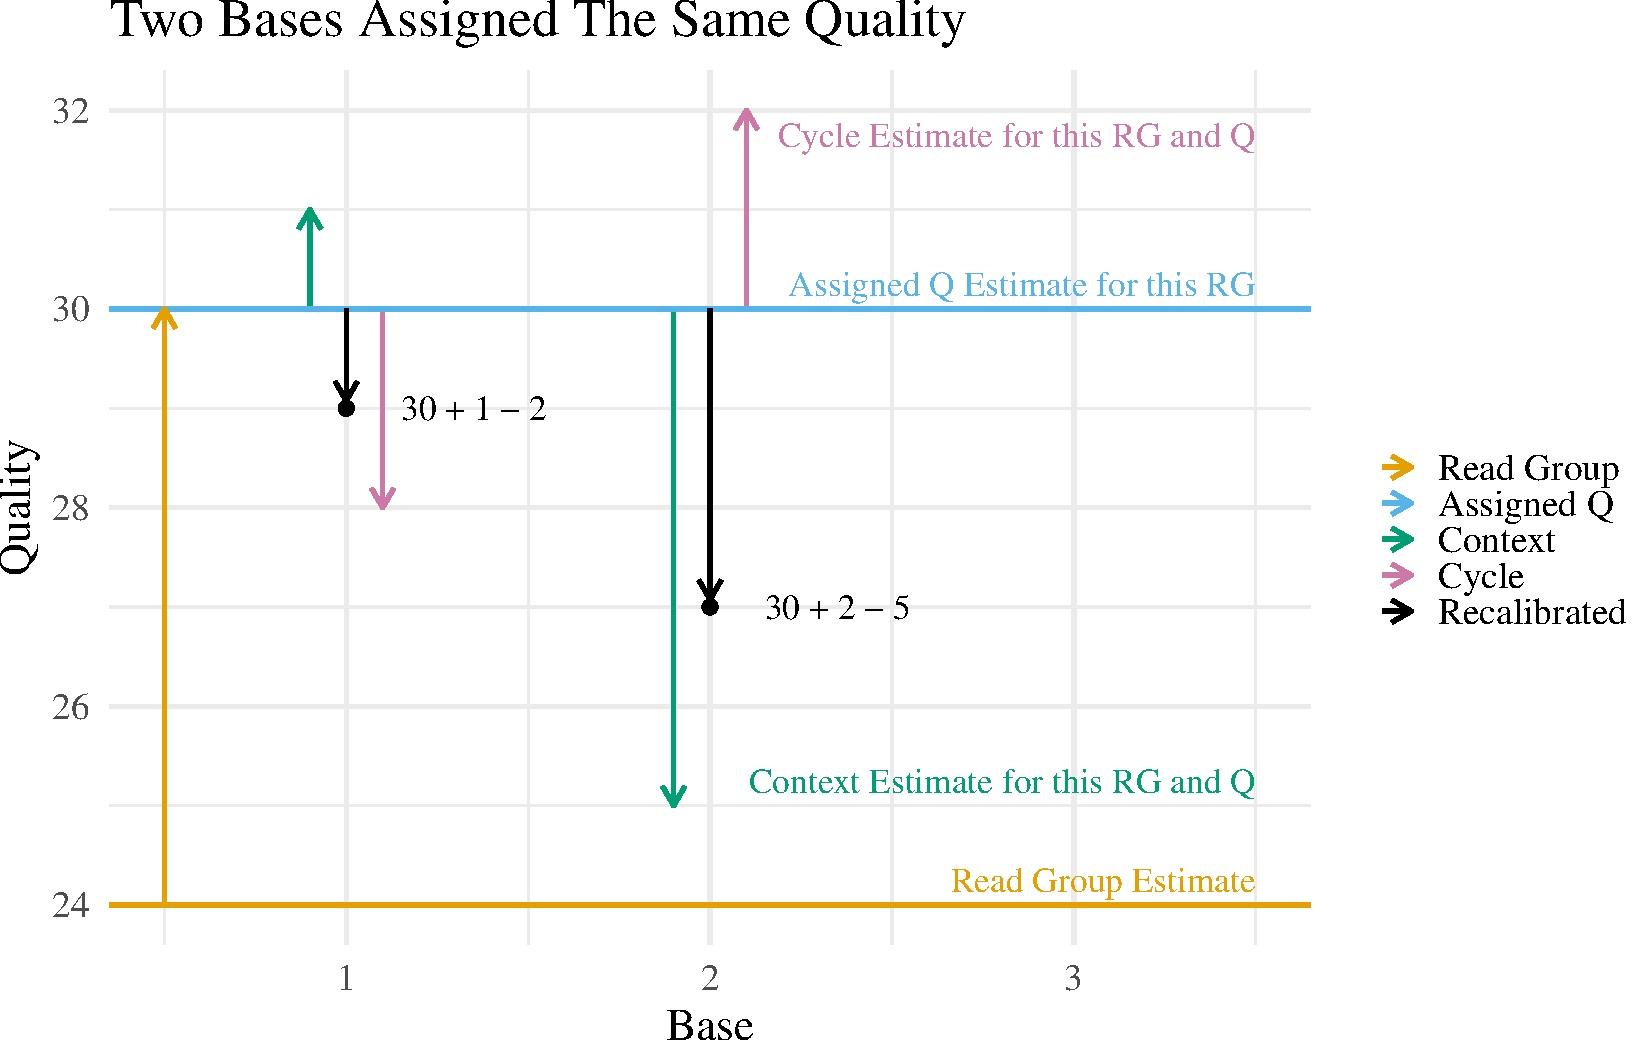
\includegraphics[width = \textwidth]{recalibration_explainer.pdf}
	\titlecaption{Base Quality Score Recalibration Example}{An example of two bases that were assigned identical quality scores. Here, the read group has an estimated quality of 24 and the assigned quality score in that read group has an estimated quality of 30. The estimated quality of bases with the same context as the first base is 31 while the estimated quality of bases with the same cycle is 28. This results in an overall estimated quality score of 29. Despite having the same read group and assigned score, because of the difference in context and cycle, the second base is assigned a different score.}
	\label{fig:recal_explain}
\end{figure}


% How much does BQSR help?
BQSR improves quality score calibration in many cases, especially when there is moderate sequencing depth and the database of variable sites is nearly complete. %todo : cite
While BQSR is recommended in GATK's Best Practices, its effect on the resulting variant calls is not well-characterized, and there is ongoing debate about whether to continue recommending BQSR. \parencite{van_der_auwera_geraldine_2020, van_der_auwera_geraldine_2020_b}
However, \textcite{ni_improvement_2016} find that improved quality score calibration aids detection of minor alleles in high coverage datasets by increasing sensitivity and reducing the number of false positive calls.
Thus, the need to perform BQSR and the performance of GATK's BQSR algorithm may vary from study to study.
Two objectives of this work are to help elucidate when GATK BQSR performs well and when it fails and to provide a method that works in situations that GATK BQSR struggles with.
As an example, the GATK developers recommend BQSR for use in cancer variant discovery \parencite{cibulskis_sensitive_2013}, but the tumor genome is likely much different from the human genome, and the database of variable sites will likely miss many truly variable sites due to the large mutation rate present in cancer genomes. Additionally, mismatches in reads misaligned due to chromosomal rearrangements may be mistakenly counted as evidence of sequencing error. The number of these errors required to significantly impact the performance of the algorithm is not clear.

\subsection{Alternate Approaches for BQSR}
% What is the problem with current methods for BQSR?
As illustrated above, the most problematic aspect of GATK BQSR occurs in the first phase of the algorithm: counting erroneous and non-erroneous bases. This is especially true when considering non-model organisms, where alignment errors may be common. Furthermore, in non-model organisms a database of variable sites is likely unavailable or largely incomplete. However, there are methods that attempt to overcome this deficiency. While there exist alternative approaches that implement different error models such as Lacer \parencite{chung_lacer:_2017}, the biggest problem for analyzing data without reliable reference information is the method of counting erroneous and non-erroneous bases.
% \item In a variant calling context, BQSR is probably most helpful in regions with low coverage, as the limited amount of data makes it difficult to differentiate between errors, heterozygous sites, and mutations.
 % or inconsistent coverage, as one may expect when sequencing a non-model organism; however, by definition that means no quality reference nor database of variable sites are available. Since these are required to perform GATK's BQSR, that means BQSR cannot be confidently completed.
% \item Find some estimates of differences between reference and samples sequenced; perhaps look at mouse
% \item This will be highly species-dependent and situation specific

% Alternative Approaches
Many alternative algorithms have been developed to avoid providing a database of variable sites. However, these approaches all still require a reference and alignment, and many require extra reagents and sequencing spike-ins that increase the cost of analysis and cannot be used to reanalyze existing sequencing data that hasn't been specially prepared.
% \item Lacer \parencite{chung_lacer:_2017} bins aligned bases based on depth and whether the base matches the reference, then uses singular value decomposition to infer the shift in quality score for each base.
ReQON \parencite{cabanski_reqon:_2012}, like GATK, considers bases that do not match the reference as errors but limits the number of acceptable errors at a position to minimize the effect of unknown variants. It then uses a logistic regression to recalibrate the quality scores.
SOAP2 \parencite{li_soap2:_2009} contains a model for consensus sequence construction that performs BQSR during construction. %It doesn't seem possible to get these recalibrated scores out??
The methods of \textcite{zook_synthetic_2012} and \textcite{ni_improvement_2016} use synthetic spike-ins of known composition and GATK's model \parencite{zook_synthetic_2012} or piecewise regression \parencite{ni_improvement_2016} to recalibrate quality scores. Since the sequence of the spike-in is known before hand, errors are easy to identify as there should be no biological variation in the spiked-in sample.
% \item While these approaches are useful alternatives to GATK, the comparisons presented here will only compare against GATK BQSR as none of the alternative approaches function without a reference and GATK BQSR is the most popular method.
Crucially, these methods require a reference and possibly other information to recalibrate reads that may not be available.

% kbbq
To effectively recalibrate base quality scores with as little auxiliary information as possible, I developed KBBQ, a software package to recalibrate quality scores of whole genome sequencing data without a reference or database of variable sites. The only required input is the set of reads to be recalibrated. Rather than excluding variation and comparing to the reference like GATK does, KBBQ uses k-mer subsampling to find likely errors. Once the number of errors and nonerrors are counted and categorized according to their covariates, it uses the same model GATK uses to recalibrate the reads. Here, I show that this difference in how KBBQ and GATK detect sequencing errors impacts the resultant base quality scores and that KBBQ produces superior calibrations in a variety of scenarios.

\section{Methods}
	% \item Error correction algorithms
KBBQ performs BQSR by adjusting how errors in the dataset are discovered.
Instead of looking at the reference, KBBQ implements the error-correction algorithm described in \textcite{song_lighter_2014} and uses the errors detected by that procedure to train and apply the standard GATK model. Note that the sequenced bases are not actually changed; the detected errors are used only to train the model. If there is evidence according to the model that the base is erroneous, its base quality will be decreased according to the strength of that evidence.

Briefly, the algorithm subsamples k-mers from the dataset. Since erroneous k-mers are expected to be unique, erroneous k-mers are less likely to be sampled than error-free k-mers. A binomial test is then conducted for every nucleotide in the dataset; if a sufficient number of k-mers contain the nucleotide, the base is likely not erroneous and called trusted. If \textit{k} of these trusted bases appear next to each other, that k-mer is stored as a trusted k-mer. Once the trusted k-mers have all been stored, each read is iterated through once again and any bases on the edge of an island of trusted k-mers are changed such that the change produces the maximal number of trusted k-mers in the read. These changes are marked as errors and used to train the model.
The model training and recalibration procedure are the same as those described above for GATK's BQSR method.

\subsection{KBBQ Program Input and Parameters}

KBBQ requires as input a set of reads in FASTQ \parencite{cock_sanger_2010} or BAM \parencite{li_sequence_2009} format. If the input data is FASTQ formatted and consists of multiple read groups, the read group each read belongs to should be annotated in the name of each read. Alternatively, if the user has an original data file and a data file that has already been corrected using an error correction program, the user may supply the corrected file with the \texttt{-\phantom{}-fixed} option to obtain errors from that correction rather than performing the error correction algorithm included in KBBQ. The program's only required parameter is the approximate length of the sequenced region in base-pairs, and this information can be taken from the BAM header if it is present. It may be set with the \texttt{-\phantom{}-genomelen} option. If BAM input is provided, the \texttt{-\phantom{}-set-oq} and \texttt{-\phantom{}-use-oq} flags can be used to set the OQ flag on the read before recalibrating or to use the quality scores encoded in the OQ flag rather than the quality scores in the primary quality score field.

Optionally, the approximate sequencing coverage may also be provided with the \texttt{-\phantom{}-coverage} option. If it is not, it will be estimated by finding the length of the sequenced data divided by the provided genome length; $\operatorname{Coverage} = \frac{\operatorname{Sequence\:Length}}{\operatorname{Genome\:Length}}$.
An $\alpha$ parameter may also be provided with the \texttt{-\phantom{}-alpha} option; this is the same $\alpha$ parameter that Lighter uses, and is the fraction of reads sampled from the input data \parencite{song_lighter_2014}. If not provided, the recommended value of $\alpha = \frac{7}{\operatorname{Coverage}}$ is used.
A $\texttt{-k}$ parameter may also be provided, which changes the k-mer size used for the error detection algorithm. The maximum value of 32 is recommended and is the default value.
A summary of flags and options the program supports is listed in table \ref{table:params}.

%new para
The genome length parameter, in addition to being used to estimate sequencing coverage, is also used to estimate the number of k-mers that will be sampled. This is used to parameterize the bloom filter that stores the sampled and trusted k-mers. This parameterization is different than that used in Lighter; there, the number of sampled k-mers is estimated to be $1.5 \times \operatorname{Genome\:length}$. However, the expected number of sampled k-mers $K_{\operatorname{sampled}}$ is bounded by the expected value of the binomial distribution parameterized by $\operatorname{Genome\:length} \times \operatorname{Coverage}$ and $\alpha$. Assuming \textit{every} k-mer is unique, the number of possible k-mers in the dataset $K_{\operatorname{total}}$ is less than $\operatorname{Coverage} \times \operatorname{Genome\:length}$. Since the number of k-mers in each read is $\operatorname{Read\:length} - k + 1$ and assuming equal read lengths, the total number of k-mers is:
\begin{align}
K_{\operatorname{total}} &= \sum_{\operatorname{Reads}}{\operatorname{Read\:length} - k + 1} \\
&= (\operatorname{Read\:length} - k + 1) \times \operatorname{Number\:of\:reads} \\
&< \operatorname{Read\:length} \times \operatorname{Number\:of\:reads} \\
&< \operatorname{Read\:length} \times \frac{\operatorname{Coverage} \times \operatorname{Genome\:length}}{\operatorname{Read\:length}} \\
&< \operatorname{Coverage} \times \operatorname{Genome\:length}
\end{align}

So the expected number of sampled k-mers is

\begin{align}
E[K_{\operatorname{sampled}}] &= E[\mathcal{B}(x; \alpha, K_{\operatorname{total}})] \\
&= \alpha \times K_{\operatorname{total}} \\
&< \alpha \times \operatorname{Coverage} \times \operatorname{Genome\:length}
\end{align}

Notably, if $\alpha$ is the recommended value of $\frac{7}{\operatorname{Coverage}}$, the expected number of sampled k-mers is less than $7 \times \operatorname{Genome\:length}$, a bound over 4 times larger than the estimate used by Lighter. For the data analyzed here, this provides a much better estimate of the true number of sampled k-mers. Ultimately, the larger estimate of elements inserted into the bloom filter causes an increase in size of the bloom filter but a smaller false positive rate.

\begin{table}
\centering
\begin{tabularx}{\textwidth}{ l  l >{\hsize=.7\hsize\linewidth=\hsize}X >{\hsize=1.3\hsize\linewidth=\hsize}X }
\toprule
\textbf{Parameter} & \textbf{Short Option} & \textbf{Default Value} & \textbf{Summary} \\
\midrule
\texttt{-\phantom{}-ksize} & \texttt{-k} & 32 & Size of k-mer to use for correction\\
\texttt{-\phantom{}-use-oq} & \texttt{-u} & Off & Use BAM OQ tag values as quality scores\\
\texttt{-\phantom{}-set-oq} & \texttt{-s} & Off & Set BAM OQ tag values before recalibration\\
\texttt{-\phantom{}-genomelen} & \texttt{-g} & Estimated for BAM, required for FASTQ & The approximate size of the sequenced region in base-pairs.\\
\texttt{-\phantom{}-coverage} & \texttt{-c} & Estimated from data & Approximate sequencing coverage\\
\texttt{-\phantom{}-fixed} & \texttt{-f} & Off & Treat changes to reads in the given file as errors and recalibrate. \\
\texttt{-\phantom{}-alpha} & \texttt{-a} & 7 / coverage & Rate to sample k-mers\\
\texttt{-\phantom{}-threads} & \texttt{-t} & 1 & Number of CPU threads to use\\
\bottomrule
\end{tabularx}
\titlecaption{KBBQ Parameters}{Provides the short options for each long parameter name, the default value of the parameter and a summary of how each parameter changes the behavior of the program.}
\label{table:params}
\end{table}

\subsection{Testing and Validation}
% Describe test dataset used for benchmarking.
To test the performance of KBBQ, I reanalyzed the synthetic diploid CHM1-CHM13 dataset from \textcite{li_synthetic-diploid_2018} (SRA accession ERR1341796, aligned to hg19). Like other benchmarking datasets, this dataset includes a BED file describing confident regions in which the genotype of any site that differs from homozygous reference within those regions are included in a VCF file. For the purposes of this work, I assume these confident regions and associated VCF entries are correct and represent the true genotype of the sequenced sample.

This dataset was specifically designed to study the impact of deep sequencing on variant calling and has a coverage of approximately 45x. Thus, the effect of sequence specific errors and other non-random biases in sequencing should be pronounced in this data.
The dataset was constructed by adding equal concentrations of DNA of CHM1 and CHM13 human complete hydatidiform mole cell lines and sequencing the mixture. These moles are formed when a sperm combines with an egg containing no nucleus; the sperm then undergoes mitosis to generate a completely homozygous cell mass. They are effectively haploid, and it is significantly easier to genotype a haploid cell than a diploid one. Thus, the mixture simulates a diploid human cell but the genotype of each haplotype is known. This means there should be very few, if any, errors in the declared genotypes included with the data, and this was confirmed by \textcite{li_synthetic-diploid_2018}.

%new paragraph
To measure the performance of KBBQ and compare to GATK's BaseRecalibrator and ApplyBQSR tools, I subset the full dataset to only reads aligned on Chromosome 1 and overlapping the BED of confident regions using the samtools view command \parencite{li_sequence_2009} and the -L parameter. I then used the samtools (version 1.10) view command with the -F 3844 flag to remove unmapped, secondary, and supplementary alignments as well as reads marked as failing quality checks and as PCR duplicates. I then used the fixmate and view commands with flag -f 1 to remove any singleton reads. I then ran KBBQ (commit ID 9167b72599892a33493d8ebdc01fac33990c1738) on the dataset with the options \texttt{-\phantom{}-use-oq -g 214206308 -a .15}. I also ran GATK (version v4.1.8.0-5-g1836ab0-SNAPSHOT) BaseRecalibrator with the provided variant data as the known sites file and the \texttt{-\phantom{}-use-original-qualities} flag set. I then used the ApplyBQSR tool with the \texttt{-\phantom{}-use-original-qualities} flag to recalibrate the input file. The \texttt{-\phantom{}-use-original-qualities} flag is appropriate here because the data has already been recalibrated and the original assigned quality scores are stored in the OQ tag on each of the reads. This flag tells GATK to use and recalibrate those quality scores, rather than using the scores that are already present in the QUAL field for the read.

I then compared the two recalibrated files by running the BaseRecalibrator tool again on both output datasets. In this invocation of BaseRecalibrator, \texttt{-\phantom{}-use-original-qualities} was not set as the quality scores in the QUAL field of the recalibrated reads are the quality scores calculated using the models trained above. I then used GATK's AnalyzeCovariates tool to create CSV files containing the number of errors for each assigned quality scores and plotted these values.

% GATK chimp test
To simulate a situation where a researcher has sequenced a non-model organism, is using a reference that may not closely match the sample, and doesn't have a database of variable sites, I aligned the test data to the chimp reference genome \parencite{waterson_initial_2005} using NextGenMap \parencite{sedlazeck_nextgenmap_2013} version 0.5.2 with the -p flag as the reads are paired. Prior to realignment, the original qualities in the OQ tag were placed into the QUAL field using GATK's RevertBaseQualityScores tool to ensure the raw assigned quality scores were used to align the reads.

In this situation, GATK recommends calling an initial set variants with high confidence and using these variants as the database of variable sites. %todo: give GATK parameters, etc used.
To see how this affects the results of GATK's BQSR, I called variants using HaplotypeCaller with the \texttt{-stand-call-conf 50} argument. The default value for this argument is 40, and is a phred-scaled confidence threshold for reporting a variant, so with this flag the model's confidence in the emitted calls should be very high. I then used the resulting variants as the database of variable sites with BaseRecalibrator to train a recalibration model. Here, the \texttt{-\phantom{}-use-original-qualities} flag was not used as the qualities in the QUAL field for each read were already the raw uncalibrated scores.

To evaluate this model using the truth set, I used the model and ApplyBQSR to recalibrate the reads as they were aligned to the human reference. Here, the \texttt{-\phantom{}-use-original-qualities} flag was used, as the quality scores that represent the original assigned scores for the reads (the same scores used to train the model) are given in the OQ tag rather than the QUAL field. Since the recalibration was performed after the reads were already aligned to the human reference, the sole difference between this recalibration method and the standard using the correct reference and database of variable sites is the trained model; the alignment has no impact on benchmarking the calibration. I then used AnalyzeCovariates as above to obtain the calibration data and plot it.

% Simulated Reads
As an additional test of KBBQ's performance, particularly in situations where the user has no quality reference, I simulated reads from the unscaffolded contigs of the initial release (v1.0) of the \textit{Eucalyptus grandis} genome, SRA accession AUSX00000000.1. GATK recommends using at least 100 million base pairs for calibration, so I aimed to simulate twice that many bases. To simulate a situation where a user has a medium-coverage dataset of approximately 20X coverage, I therefore simulated a haploid genome of 5 million base pairs by randomly sampling contigs from the full set of \textit{E. grandis} contigs using shuf, awk, and the samtools faidx program.

I then simulated heterozygous sites in the genome using simuG version 1.0.0 \parencite{yue_simug_2019} with a transition/transversion ratio of 2 to mirror the approximate ratio of mutations in real eucalypts. I simulated 125,000 SNPs in the reference to reflect the large level of heterozygosity in eucalypts \parencite{kulheim_comparative_2009}. I then concatenated the subsampled reference and reference containing the SNPs, which I used to simulate 101-bp long paired end reads using ART (version MountRainier-2016-06-05; \cite{huang_art_2012}) using the HiSeq 2500 error profile, a mean fragment length of 300, a fragment length standard deviation of 20, and a depth of coverage of 20. Since this concatenated genome is twice the size as the haploid genome, at 20 fold coverage it would yeild approximately 200 million base-pairs of sequence. I then aligned the simulated reads to the genome with NextGenMap \parencite{sedlazeck_nextgenmap_2013}.

This reflects a scenario where a researcher sequences a highly heterozygous individual, assembles contigs, and aligns the sequenced reads back to the assembly. However, in this case the locations of all heterozygous sites are known. To compare the performance of KBBQ and GATK recalibration, I built the recalibration model with GATK BaseRecalibrator using the true location of all the heterozygous sites and applied the model with with GATK ApplyBQSR, both without the \texttt{-\phantom{}-use-original-qualities} flag since the assigned quality scores were present in the QUAL field of the read. Since most researchers don't have knowledge of all the true variable sites in the data, I also repeated this procedure but using the initial calls made by HaplotypeCaller with the \texttt{-\phantom{}-stand-call-conf} parameter set to 50, which makes HaplotypeCaller emit only variants it is highly confident in. I then ran KBBQ using a k-mer size of 32 and a genome length of 5 million to recalibrate the reads. Finally, I used BaseRecalibrator again and GATK's AnalyzeCovariates tool with the CSV output option to check the calibration of each of the four recalibrated alignments.

%

Scripts to replicate the above analyses are available in Appendix \ref{ch:kbbq_plot_code}.

\section{Results}

Using GATK's recommended method of using high-confidence variants when a database of variable sites is unavailable produced poorly calibrated data with a RMSE of 3.89. The shape of this recalibrated data is also interesting; it shows that the quality scores are underconfident for mid-range quality scores and overconfident for high quality scores. This calibration and the calibration using the true set of variants, using KBBQ, and the raw read quality are plotted in Figure \ref{figure:comparison} and the RMSEs of each data set is listed in Table \ref{table:comparison}

\begin{figure}
\centering
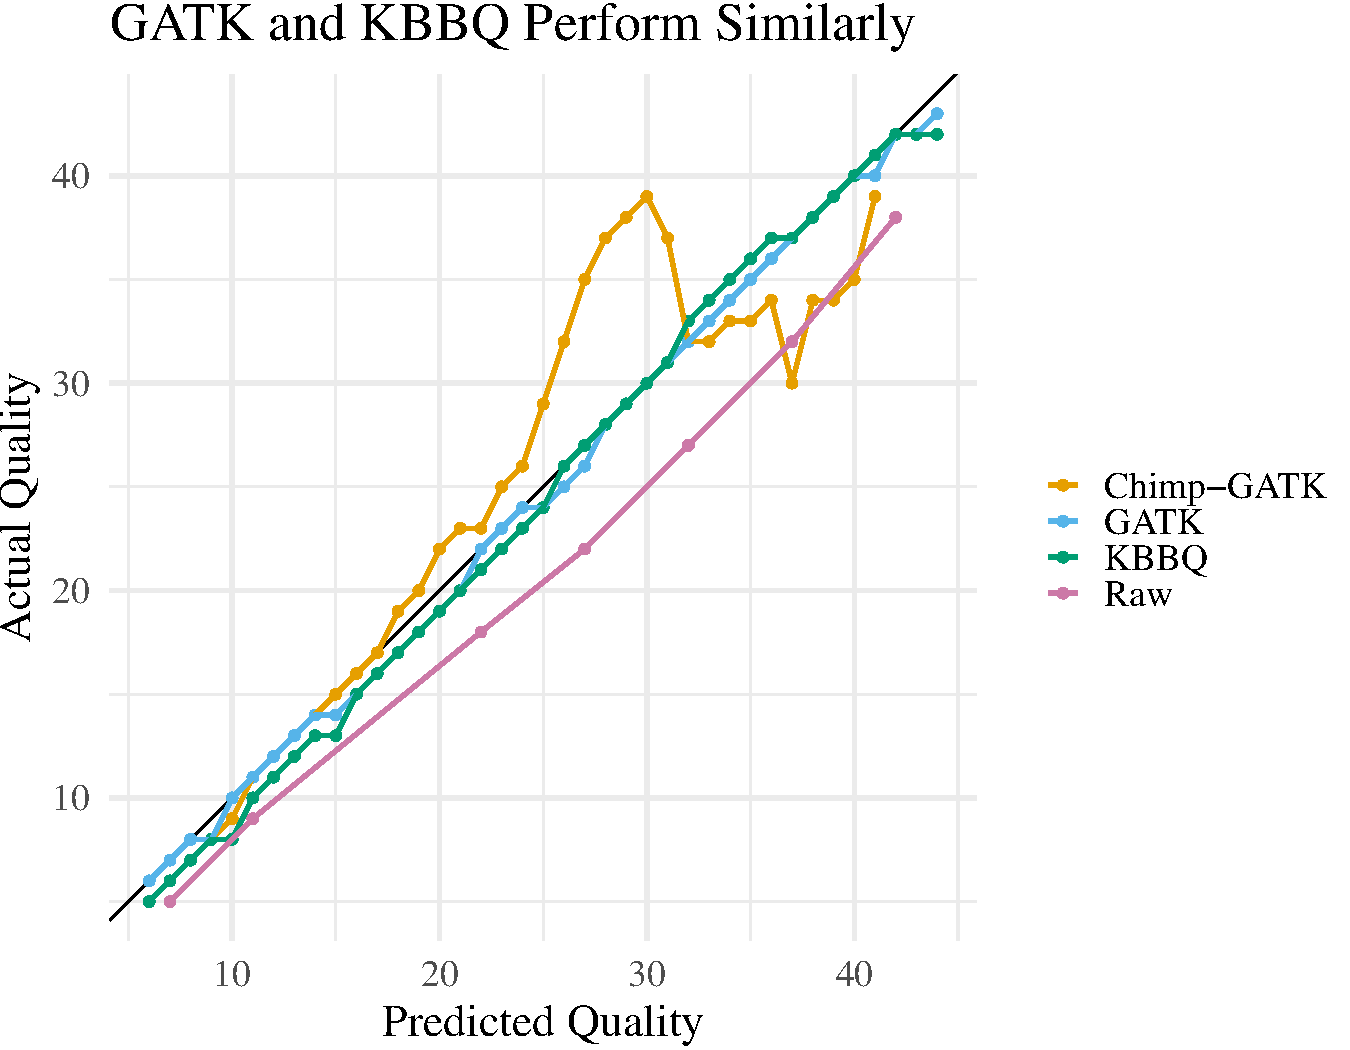
\includegraphics[width = .6\textwidth]{comparison.pdf}
\titlecaption{Comparison of Calibration Methods}{Chimp-GATK is the result of calibrating the reads using the model trained on the reads aligned to the chimp genome along with the variants called using that alignment. GATK is the result of using GATK's BaseRecalibrator with the truth set of variants. KBBQ is the result of using the KBBQ tool, which requires only reads and no reference or variant set. Raw is the calibration of the uncalibrated data.}
\label{figure:comparison}
\end{figure}

\begin{table}
\centering
\begin{tabular}{r l}
\toprule
Calibration Method & RMSE \\
\midrule
Chimp-GATK & 3.89 \\
GATK & 0.60 \\
KBBQ & 0.96 \\
Raw & 4.05 \\
\bottomrule
\end{tabular}
\titlecaption{Errors of Different Calibration Methods}{Root mean squared error of quality score for reads recalibrated using different methods. Chimp-GATK is the result of calibrating the reads using the model trained on the reads aligned to the chimp genome along with the variants called using that alignment. GATK is the result of using GATK's BaseRecalibrator with the truth set of variants. KBBQ is the result of using the KBBQ tool, which requires only reads and no reference or variant set. Raw is the calibration of the uncalibrated data.}
\label{table:comparison}
\end{table}

The resulting calibration of each recalibration method applied to the simulated data is shown in Figure \ref{fig:sim_comparison}. The raw data as simulated is fairly well-calibrated and almost all quality scores are on the 1-to-1 line. GATK recalibration with an initial callset caused calibration errors in high scoring bases. GATK recalibration caused a large calibration error for bases assigned a score of 20, which contained very few errors. However, there were also relatively few bases assigned a score of 20, as seen in Figure \ref{fig:sim_qual_counts}. The errors are summarized in Table \ref{table:sim_comparison}; KBBQ has the lowest RMSE, while GATK calibration using an initial HaplotypeCaller callset has the highest RMSE.

\begin{figure}
\centering
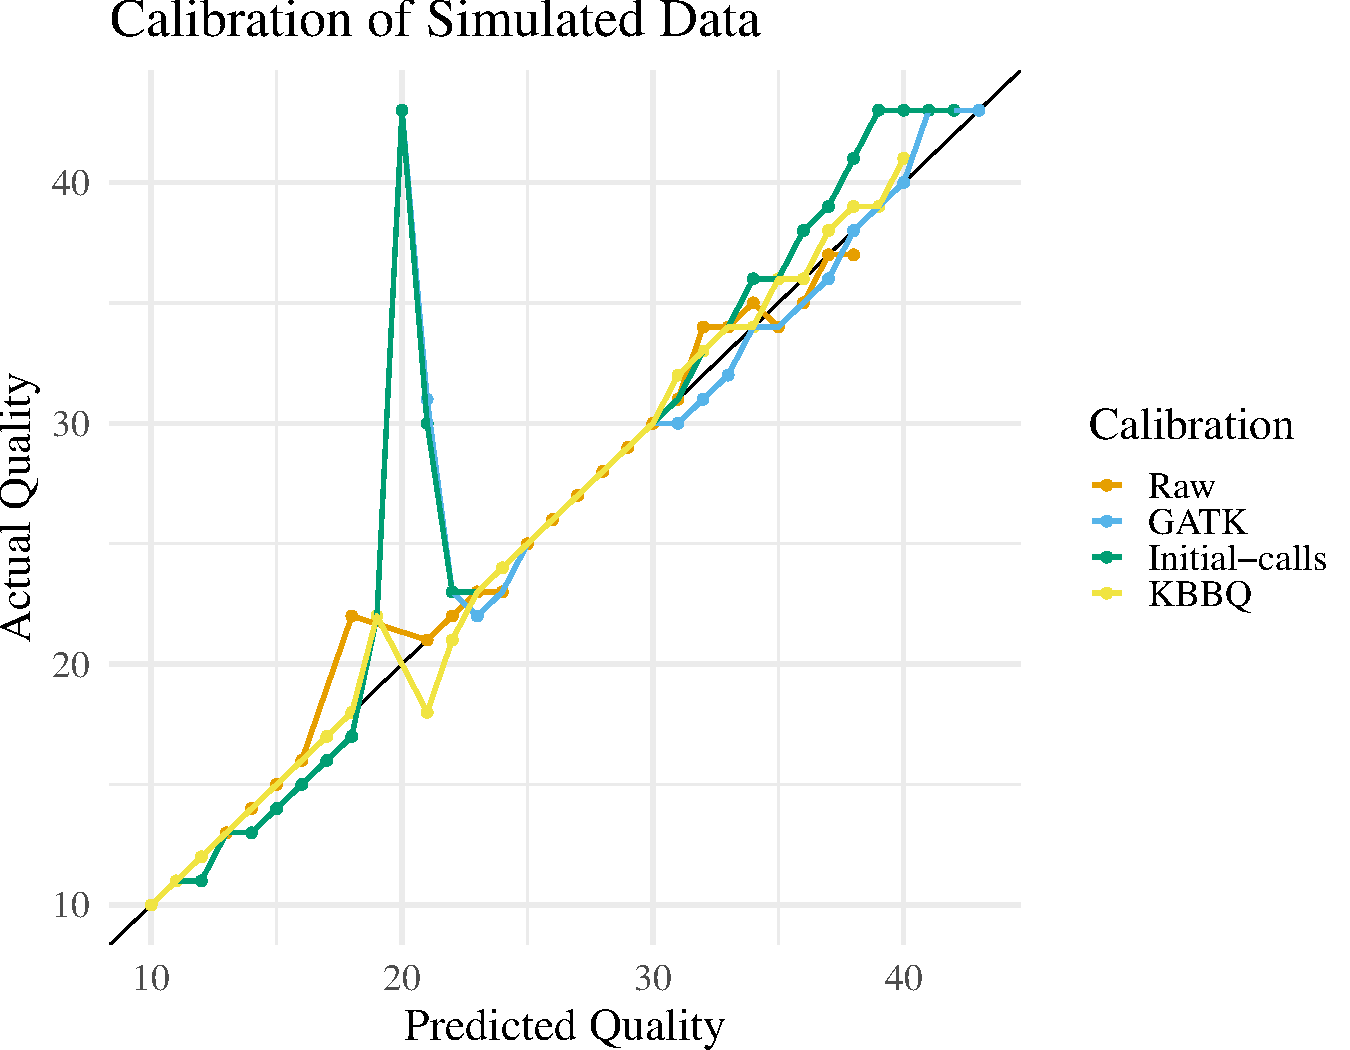
\includegraphics[width = .6\textwidth]{sim_comparison.pdf}
\titlecaption{Comparison of Calibration Methods on Simulated Data}{Plot of calibration errors before and after recalibrating reads simulated with ART. Raw is the unmodified simulated quality scores. GATK is the result of using BaseRecalibrator and ApplyBQSR using the set of true simulated variants as the known sites file. Initial-calls is the result of using BaseRecalibrator and ApplyBQSR but using an initial HaplotypeCaller callset rather than the true set of variants. KBBQ is the result of using KBBQ, a reference-free recalibration method. Note that the raw calibration lies almost all on the 1-to-1 line, meaning the data is already fairly well-calibrated.}
\label{fig:sim_comparison}
\end{figure}

\begin{figure}
\centering
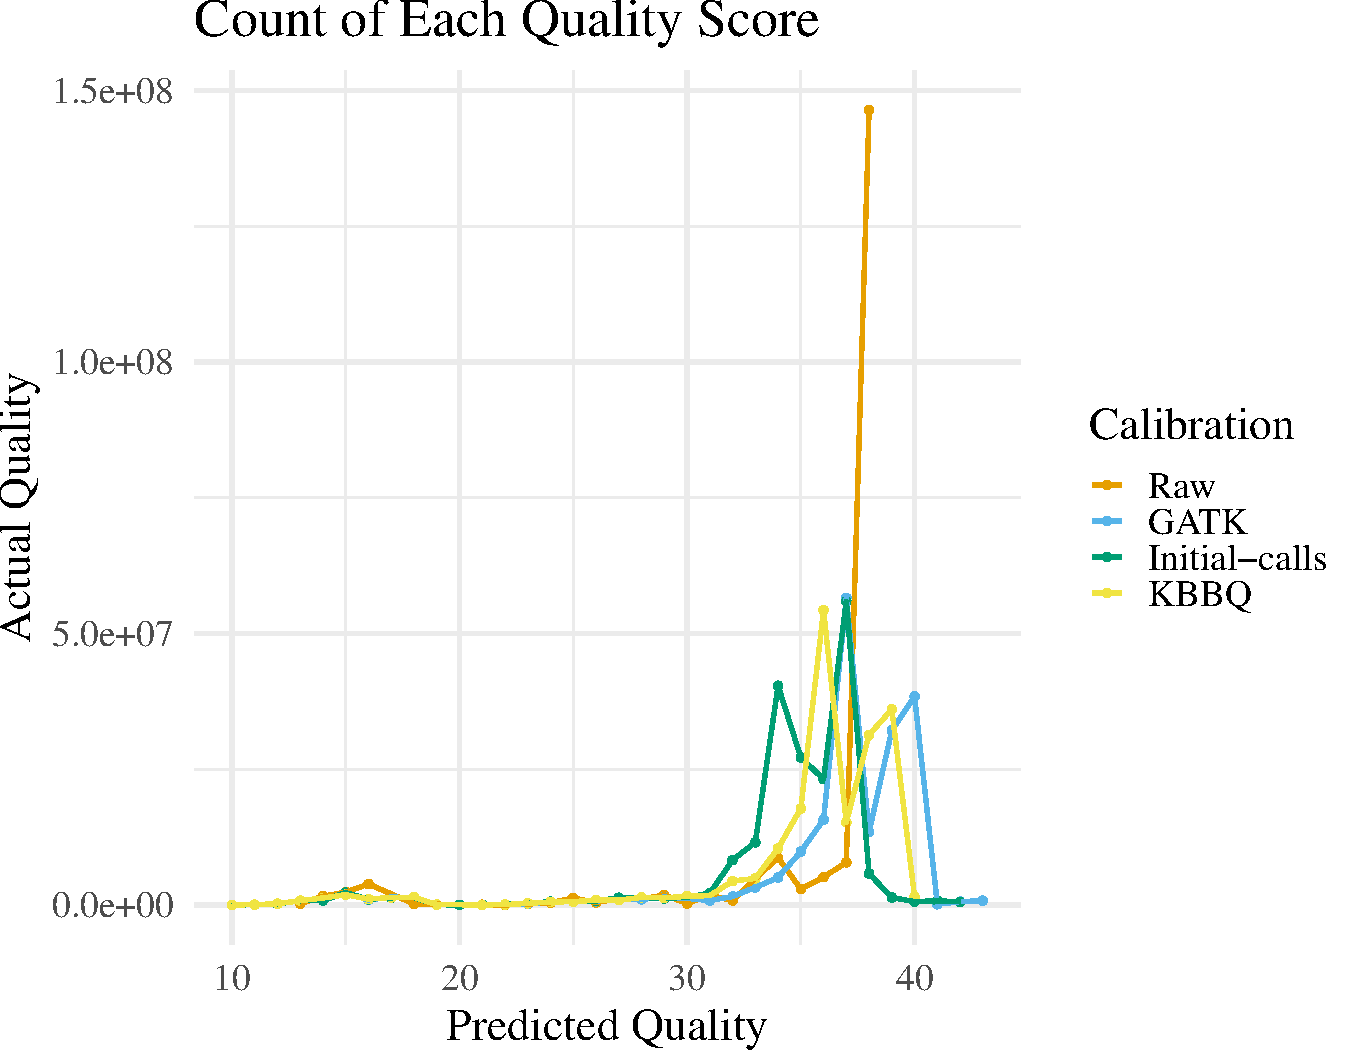
\includegraphics[width = .6\textwidth]{sim_qual_counts.pdf}
\titlecaption{Quality Score Distribution of Recalibrated Simulated Data}{Plot of the counts of each quality score in each dataset recalibrated by different methods. Raw is the unmodified simulated quality scores. GATK is the result of using BaseRecalibrator and ApplyBQSR using the set of true simulated variants as the known sites file. Initial-calls is the result of using BaseRecalibrator and ApplyBQSR but using an initial HaplotypeCaller callset rather than the true set of variants. KBBQ is the result of using KBBQ, a reference-free recalibration method. Most quality scores are above 30, and all the recalibration methods yield a distribution near that mode.}
\label{fig:sim_qual_counts}
\end{figure}

\begin{table}
\centering
\begin{tabular}{r l}
\toprule
Calibration Method & RMSE \\
\midrule
Raw & 1.06 \\
GATK & 4.40 \\
Initial-calls & 4.54 \\
KBBQ & 0.93 \\
\bottomrule
\end{tabular}
\titlecaption{Errors of Different Calibration Methods on Simulated Data}{Root mean squared error of quality score for simulated reads recalibrated using different methods. Raw is the unmodified simulated quality scores. GATK is the result of using BaseRecalibrator and ApplyBQSR using the set of true simulated variants as the known sites file. Initial-calls is the result of using BaseRecalibrator and ApplyBQSR but using an initial HaplotypeCaller callset rather than the true set of variants. KBBQ is the result of using KBBQ, a reference-free recalibration method. See Figure \ref{fig:sim_comparison} for a visualization of the calibration errors.}
\label{table:sim_comparison}
\end{table}

\section{Discussion}
%Rewrite this given we moved most the hapdip stuff to ch5

% At the same time, the calibration model trained with the chimp-aligned data shows performance worse than a simulated dataset with a false negative rate around 40-60\%. The RMSE of 3.89 is only slightly better than the RMSE of the raw data and the plotted calibration shows very poor performance at higher quality scores. Additionally, quality scores assigned between 25 and 32 were significantly different than the true quality scores. And while all the simulated datasets caused underconfidence in the calibration, this calibration method caused overconfidence in quality scores above 34.
% This suggests that an effect not captured in the simulated data was present in this data. Overconfidence indicates errors that should be counted by the model are instead missed and therefore there are more errors in actuality than the model predicts. Thus the set of variants used to skip errors is too aggressive and contains many false positives. So why is a similar effect not observed in the simulated data?
% This overconfidence is observed in the Chimp-GATK calibration method.
As the chimp-aligned calibration shows, GATK BQSR struggles to accurately recalibrate quality scores when the reference doesn't closely match the sample. This could cause issues when attempting to use GATK BQSR on data from a non-model organism if the reference contains errors or is otherwise distant to the sampled organism. False negatives are likely to be numerous in almost all but the most well-studied samples \parencite{bobo_false_2016}, and false positives are similarly likely when using poor quality, draft reference genomes that cause alignment errors. This means in many datasets, while its performance may be acceptable if the false negative and false positive rate are sufficiently low, GATK BaseRecalibrator may not the best recalibration method. This is shown in Figure \ref{figure:comparison}, which shows KBBQ performing nearly as well as GATK BQSR with perfect knowledge of variable sites. However, KBBQ doesn't use any reference or any variant site information to do recalibration. KBBQ also performs much better than GATK's recommended procedure when a database of variable sites is not available, as shown in the Chimp-GATK calibration.

Recalibration of the simulated reads shows that KBBQ is able to recalibrate reads even if they are already well-calibrated without severely damaging the calibration of the quality scores. In contrast, using GATK---even with an accurate database of variable sites---introduces additional error in quality score calibration to the reads, with both GATK-based methods having much higher RMSE than the raw quality scores. Additionally, even though the reads were already fairly well-calibrated, KBBQ recalibration confers a slight improvement to the RMSE of the quality scores. All methods yielded quality scores near 38, the mode of the raw quality data.

% While there is a large spike in calibration error for bases assigned a score of 20, most of the data is assigned a score around 38, which is the mode of the raw data. This spike is a large contributor to the RMSE, but doesn't represent a very significant difference to the overall quality of the calibration. However, miscalibration in bases with quality scores between 32 and 40 are likely very important for the overall quality of the calibration, since most bases are assigned scores in that range. In this range, all calibration methods except GATK using intial variant calls were fairly close.


\section{Conclusion}

Base quality score recalibration is an important procedure to ensure base quality scores are accurate before variant calling. However, the most popular method for doing BQSR is not easy to do if the sequenced organism is a non-model organism. I developed the software tool KBBQ to recalibrate base quality scores without a reference or database of variable sites to overcome these deficiencies. Since it doesn't use a database of variable sites or a reference, the quality of these resources is immaterial to the quality of the resulting calibration.

To evaluate KBBQ, I emulated GATK's procedure for calibration when a database of variable sites is unavailable by aligning a synthetic diploid human benchmarking dataset to the chimp genome and calling variants to use as the database of variable sites. This method produces a calibration worse than KBBQ. I further simulated reads from a draft assembly to simulate sequencing of a highly heterozygous non-model organism. Though the simulated data was fairly well-calibrated, GATK calibration with perfect knowledge of the heterozygous sites and using an initial set of calls introduced more error into the quality score calibration than was in the original data while KBBQ recalibration slightly reduced it. Thus, when a database of variable sites or reference is unavailable or of poor quality, KBBQ is an effective method for base quality score recalibration.

\printbibliography[segment=\therefsegment]{}

	% \item Future work: see how big the difference is in variant calls using binned quality scores, miscalibrated reads, and well calibrated reads.
